\documentclass[conference]{IEEEtran}
\IEEEoverridecommandlockouts
% The preceding line is only needed to identify funding in the first footnote. If that is unneeded, please comment it out.
\usepackage{cite}
\usepackage{amsmath,amssymb,amsfonts}
\usepackage{graphicx}
\usepackage{textcomp}
\usepackage{xcolor}
\usepackage{algorithm}
\usepackage[noend]{algpseudocode}
\usepackage{hyperref}
\def\BibTeX{{\rm B\kern-.05em{\sc i\kern-.025em b}\kern-.08em
    T\kern-.1667em\lower.7ex\hbox{E}\kern-.125emX}}
\begin{document}

\title{Dynamic Background Video Forgery Detection using Gaussian Mixture Model}

\author{\IEEEauthorblockN{Nugroho Satriyanto\IEEEauthorrefmark{1}, Rinaldi Munir\IEEEauthorrefmark{2}, Harlili\IEEEauthorrefmark{3}}
\IEEEauthorblockA{\textit{School of Electrical Engineering and Informatics} \\
\textit{Institut Teknologi Bandung}\\
Bandung, Indonesia \\
\IEEEauthorrefmark{1}nugroho.s@outlook.co.id, \IEEEauthorrefmark{2}rinaldi@informatika.org, \IEEEauthorrefmark{3}harlili@informatika.org}
}


\maketitle

\begin{abstract}
Video as evidence holds an important position in a court case and therefore the integrity of video must be proven. Various studies had been done in video forensics and most of them is only focused on a certain type of forgery, such as histogram correlation analysis that only focused on detecting temporally forged videos with static background. Improving histogram correlation analysis with foreground detection using Gaussian mixture model makes it possible to detect spatially forged videos and further improves its accuracy in detecting dynamic background video. Applying this improvement will yield a better accuracy both for detection and localization and opens up new possibility to detect spatially forged videos.
\end{abstract}

\begin{IEEEkeywords}
histogram, correlation, pixel line, forgery, Gaussian mixture model
\end{IEEEkeywords}

\section{Introduction}
Evidence has an important position in criminal case trial. Existence of evidence can be used to testify crime or innocence and therefore has potential to be misused. This misuse can be done by manipulating evidence so it tells a story that never happens.

An example of evidence that often used is video. With the development of technology, such as development of more advance recording devices, video as an evidence is easily obtained. However, the development of technology also makes the integrity of video is questioned with the development of video editing software and technique.

Nowadays, video forgery can be easily performed with such editing software. This software is usually intended for entertainment purposes but this obviously does not rule out the possibility such software used for manipulating evidence for court case.

Video forgery detection can be broadly classified into active and passive based approaches \cite{b1}. In active approach, preprocessing a video is needed to insert a mark in video like watermark or digital signature. The mark inserted in active approach will be an identifier to decide whether the video is forged. Meanwhile in passive approach there is no preprocessing in video and it need to observe certain characteristics in video to determine whether the video is forged.

\section{Fundamental Concepts}
\subsection{Digital Video}
Digital video is a representation of moving image element and voice element which represented in binary data. Unlike traditional analog video, which is captured frame by frame on a tape, digital video is recorded digitally, as ones and zeros. Since it is stored in a digital format, digital video can be recognized and edited by a computer, which is also a digital device \cite{b3}.

A digital video consist of two components, visual component and sound component. Visual component in a video represented by sequence of pictures called frame. A frame consist of pixels which is the smallest programmable color on a computer display or in a computer image.

\subsection{Video Forgery}
Video forgery is intentional modification/alteration of the digital video for fabrication \cite{b1}. Implication of it depends upon the circumstance and where it is used. Particularly in the movie, political and medical world its impact is enormous where it is used to defame a personality, hide or forge important information to falsify or conceal actual.

Sowmya et al \cite{b1} classify video forgery into three group, spatial, temporal, and spatio-temporal as shown in Fig.~\ref{forgeryclass}. Spatial attack performed on content of the frame(x-y axis) which present the visual information of the video. Whereas temporal attack performed on sequence of frames which present the sequence of events occurred in video. Meanwhile, spatio-temporal attack performed on both content of the frame and sequence of frames.

\begin{figure}[htbp]
\centerline{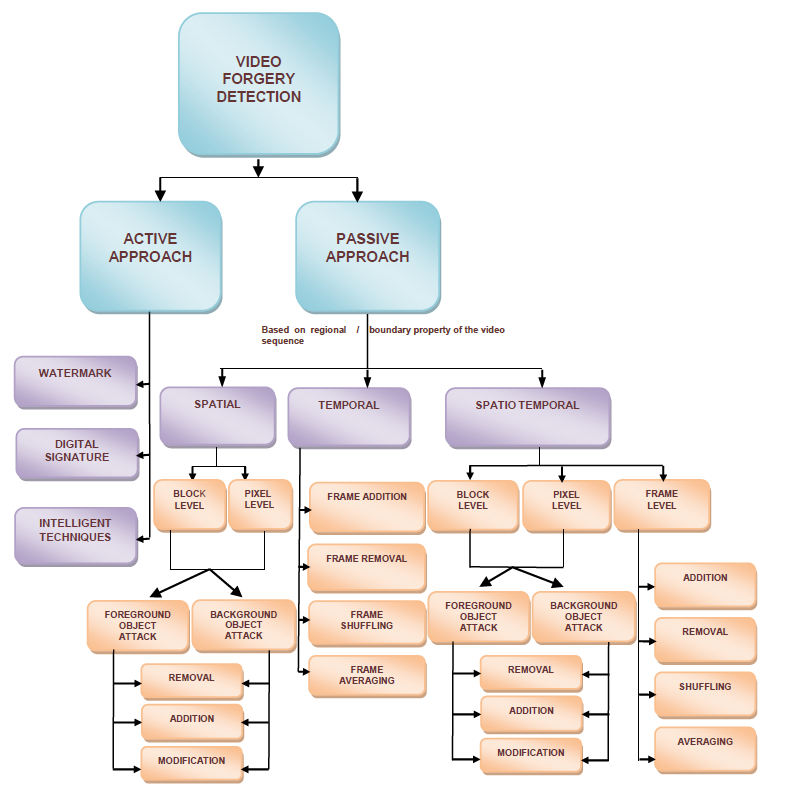
\includegraphics[width=75mm,scale=0.5]{forgeryclass.PNG}}
\caption{video forgery classification \cite{b1}}
\label{forgeryclass}
\end{figure}

\subsection{Gaussian Mixture Model}
Gaussian mixture models are a probabilistic model for representing normally distributed subpopulations within an overall population \cite{gmm}. This model does not require knowing which subpopulation a data point belongs to, and intended to determine the subpopulation automatically. Therefore, this model constitutes as unsupervised learning.

Gaussian mixture model is parameterized with two values, component weight and mean and covariance. Each component $k$ from components $K$ will have mean $\mu_k$, covariance $\sigma_k$, and weight $\phi_k$ with condition $\sum_{i=0}^k{\phi_k}=1$.

Learning process of this model commonly using expectation-maximization technique. This technique consist of two main stages, expectation for calculating the probability of a data point is a part of a cluster and maximization for recalculating model's parameters with the calculated probability.

Before the expectation stage can be performed, an initialization of model's parameter must be performed. This can be done by splitting the data randomly in K clusters then calculating the mean and covariance of each cluster. Meanwhile, the weight of each component can be assigned with $\frac{1}{k}$.

In expectation stage, the probability each data point is part of each cluster is calculated. The probability $\\gamma_{ik}$ which represents the probability of data point $i$ is part of cluster $k$ can be calculated with equation~\ref{gmmeq} and~\ref{normeq}. The maximization stage then can be performed by recalculating weight, mean, and covariance of each component with equation~\ref{weightnew},~\ref{meannew}, and~\ref{covnew}.

\begin{equation}
\gamma_{ik} = \frac{\phi_k N(x_i|\mu_k,\sigma_k)}{\sum_{j=1}^{K}{\phi_j N(x_i|\mu_j,\sigma_j)}}
\label{gmmeq}
\end{equation}

\begin{equation}
\mathcal{N}(x | \mu_i, \sigma_i) = \frac{1}{\sigma_i\sqrt{2\pi}} \exp\left(-\frac{(x-\mu_i)^2}{2\sigma_i^2}\right)
\label{normeq}
\end{equation}

\begin{equation}
\phi_k = \sum_{i=1}^N{\frac{\gamma_{ik}}{N}}
\label{weightnew}
\end{equation}

\begin{equation}
\mu_k = \frac{\sum_{i=1}^N\gamma_{ik} x_i}{\sum_{i=1}^N\gamma_{ik}}
\label{meannew}
\end{equation}

\begin{equation}
\sigma_k = \frac{\sum_{i=1}^N\gamma_{ik} {(x_i-mu_k)}^2}{\sum_{i=1}^N\gamma_{ik}}
\label{covnew}
\end{equation}

\section{Related Work}
In \cite{b2} the author proposed a method to detect video forgery based on histogram correlation between frames. The histogram is calculated from certain area in video called pixel belt. Pixel belt in video consist of several pixel lines that can be positioned horizontal or vertical. Fig.~\ref{fig1} show how pixel lines are made.
\begin{figure}[htbp]
\centerline{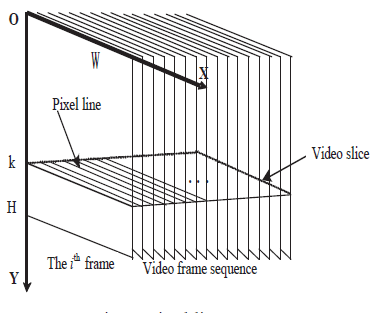
\includegraphics{pixelline.PNG}}
\caption{pixel line}
\label{fig1}
\end{figure}

Every four continuous horizontal (vertical) pixel lines make a horizontal (vertical) pixel belts. $b_h^i$ presents horizontal pixel belts and $b_v^i$ presents vertical pixel belts as defined in equation~\ref{eq1} and~\ref{eq2} where $l_h^i$ and $l_v^i$ represents $i^{th}$ horizontal and vertical pixel line and $i=1,2,3,...,L-3$ and L is the number of frame in video.
\begin{equation}
b_h^i = \left \langle l_h^i,l_h^{i+1},l_h^{i+2},l_h^{i+3} \right \rangle
\label{eq1}
\end{equation}
\begin{equation}
b_v^i = \left \langle l_v^i,l_v^{i+1},l_v^{i+2},l_v^{i+3} \right \rangle
\label{eq2}
\end{equation}

The pixel belt defined then will be iterated to count the histogram that will be compared to another histogram from other frame. $H_{b_h}^i(H_{b_v}^i)$ represents the ratio between the number of pixel with color $p$, $n_p$, with the number of pixel in pixel belt, $N$, as shown in equation~\ref{eq3} and~\ref{eq4}.
\begin{equation}
H_{b_h}^i(p) = \frac{n_p}{N}
\label{eq3}
\end{equation}
\begin{equation}
H_{b_v}^i(p) = \frac{n_p}{N}
\label{eq4}
\end{equation}

From the histogram counted then correlation,$R_{h}(i)$, can be calculated with comparing histogram from pixel belt $b_h^i(b_v^i)$ with histogram from pixel belt $b_h^{i+4}(b_v^{i+4})$ as shown in equation~\ref{eq5} and~\ref{eq6}. The correlations calculated then can be aggregated as $A_h(R)(A_v(R))$ as shown in equation~\ref{eq7} and~\ref{eq8}. The aggregated correlation then can be shown as time-series graph as shown in Fig.~\ref{corrvsframe}.
\begin{equation}
R_{h}(i) = \frac{\sum_{p=0}^{M-1}{min(H_{b_h}^i(p),H_{b_h}^{i+4}(p))}}{H_{b_h}^i(p)}
\label{eq5}
\end{equation}
\begin{equation}
R_{v}(i) = \frac{\sum_{p=0}^{M-1}{min(H_{b_v}^i(p),H_{b_v}^{i+4}(p))}}{H_{b_v}^i(p)}
\label{eq6}
\end{equation}
\begin{equation}
A_h(R) = \left \langle R_{h}(1),R_{h}(2),...,R_{h}(L-7) \right \rangle
\label{eq7}
\end{equation}
\begin{equation}
A_v(R) = \left \langle R_{v}(1),R_{v}(2),...,R_{v}(L-7) \right \rangle
\label{eq8}
\end{equation}

\begin{figure}[htbp]
\centerline{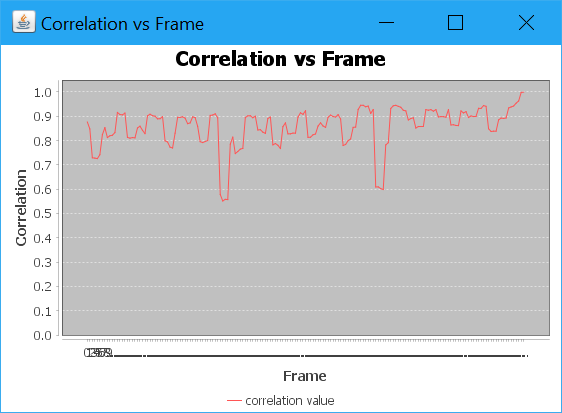
\includegraphics[width=0.9\linewidth]{corrvsframe.PNG}}
\caption{Correlation aggregate chart}
\label{corrvsframe}
\end{figure}

\begin{figure}[htbp]
\centerline{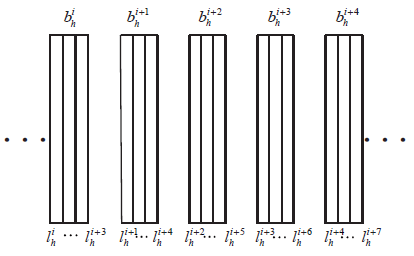
\includegraphics{pixelbelt.PNG}}
\caption{pixel belt}
\label{pixelbelt}
\end{figure}

Fig.~\ref{pixelbelt} represents a pixel belt from frame $i$ to $i+4$. If for instance frame $i+4$ is forged, then correlation $R_h(i)$ will be the minimum among $R_h(i-3)$ until $R_h(i+3)$.

To determine the location of forged frames, outlier detection must be applied. In \cite{b2}, the author used interquartile range to determine outliers. The interquartile range can be calculated with sorting the aggregate in ascending order and determining three divider based on median called $Q1$,$Q2$, and $Q3$. The outliers then can be defined as every value outside $Q1-1.5*(Q3-Q1)$ and $Q3+1.5*(Q3-Q1)$.

The problem from \cite{b2} is primarily the placement of pixel line. When the pixel line is placed in a region with minimal change as shown in Fig.~\ref{problem1} both pixel line in (a) and (b). In Fig.~\ref{problem1}(a) pixel line may cause a high correlation value because of minimal change in that region and cause a false positive. Whereas in Fig.~\ref{problem1}(b), pixel line placement can not detect changes in the circle because it does not intersect with the object and this kind of case may cause false negative.

\begin{figure}[htbp]
\centerline{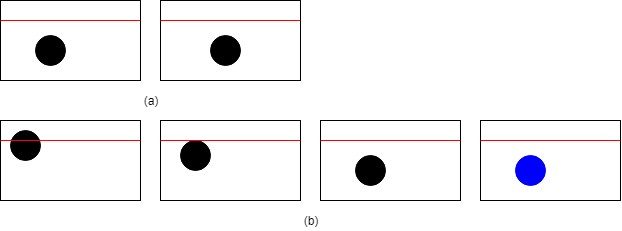
\includegraphics[width=0.9\linewidth]{problem1.PNG}}
\caption{pixel line placement problem}
\label{problem1}
\end{figure}

\section{Proposed Method}
To solve the previously mentioned problem, it is needed to place pixel line in an area that has a lot of changes. One way to do it is to use foreground detection first. Foreground detection works by detecting changes in pixel, the more a pixel changes the more likely it classified as foreground. Therefore, foreground detection is a good way to solve the problem.

The proposed method consist of six stage, foreground detection, thresholding, denoising, pixel line placement, histogram correlation calculation, and analyzing calculated correlation. These process can be represented in Fig.~\ref{sysflow}.

\begin{figure}[htbp]
\centerline{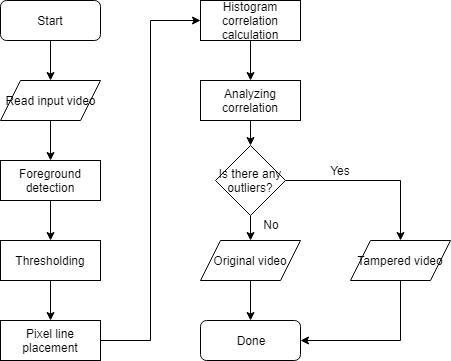
\includegraphics[width=75mm,scale=0.5]{sysflow.png}}
\caption{proposed method flowchart}
\label{sysflow}
\end{figure}

\subsection{Foreground Detection}
Main issue in dynamic background video is placing the pixel line in a location with a lot of changes. Such task can be done using foreground detection.

Gaussian mixture model can be used to do foreground detection by clustering pixels from each frame to several clusters. These clusters then can be used to determine which cluster classify as background and foreground. The probability calculated then can be used to transform video to grayscale that darker pixels more likely classify as background as shown in Fig.~\ref{gmmres}.

\begin{figure}[htbp]
\centering
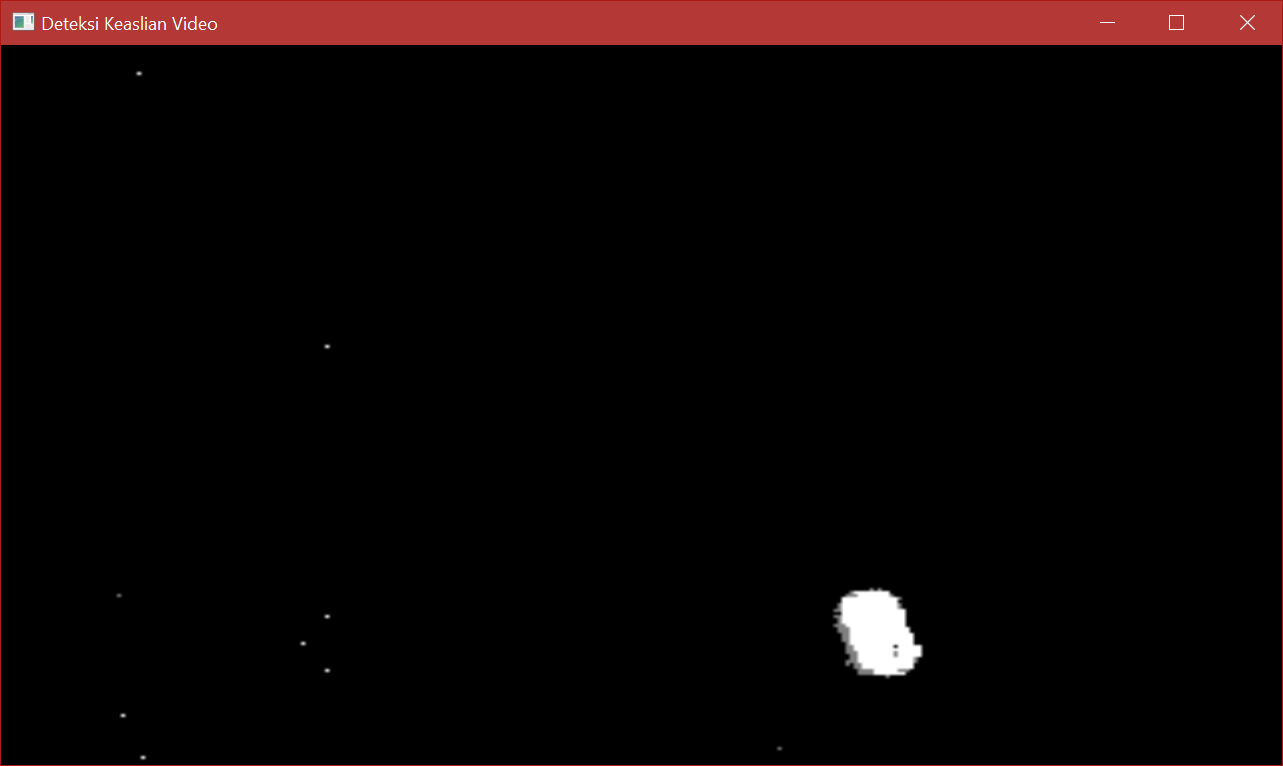
\includegraphics[width=0.9\linewidth]{gmmres.png}
\setlength\intextsep{0pt}
\caption{Grayscale video resulted from gaussian mixture model}
\label{gmmres}
\end{figure}

\subsection{Thresholding}
The result of foreground detection using gaussian mixture model is a grayscale video. Therefore, the video needs to be converted to binary video so it can be used to easily determine which pixel is a foreground.

One way to convert grayscale video to binary video is using threshold. The threshold can be used to convert all pixel value below threshold to zero or black and the other to 255 or white.

The calculation of threshold can be performed with Otsu method. This method iterates all possible threshold values then determine which threshold has the minimum distribution. The distribution between classes separated by threshold can be calculated with within-class variance $\sigma_w^2$ as shown in equation~\ref{wcv} with $q_1(t)$ represents the number of pixels below $t$, $q_2(t)$ represents the number of pixels above $t$, and $q_1(t)$ and $q_2(t)$ represent covariance of the two groups which can be calculated using equation~\ref{cv}. The result of this process will be a binary video with white pixel represents foreground pixel as shown in Fig.~\ref{thresres}.

\begin{equation}
\sigma_w^2 = q_1(t) \sigma_1^2(t) + q_2(t) \sigma_2^2(t) 
\label{wcv}
\end{equation}

\begin{equation}
\sigma_x^2 = \frac{\sigma_{i=1}^N (X_i - \mu_x)}{N}
\label{cv}
\end{equation}

\begin{figure}[htbp]
\centerline{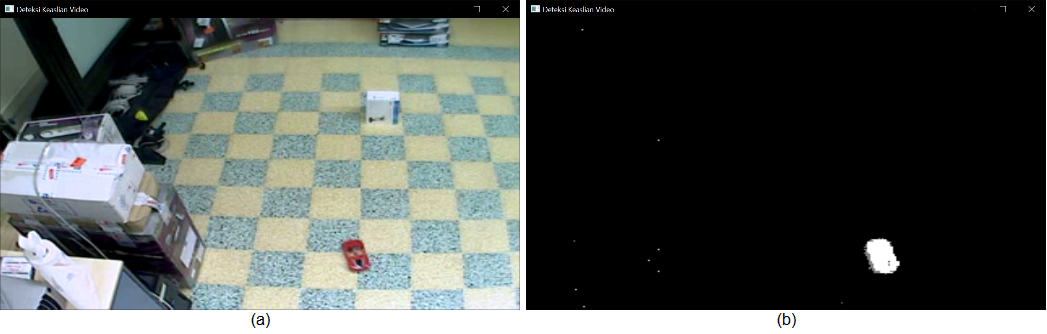
\includegraphics[width=0.9\linewidth]{thresholdres.PNG}}
\caption{thresholding result}
\label{thresres}
\end{figure}

\subsection{Denoising}
The video resulted from thresholding process will contains noises introduced by the insignificant movement of dynamic background. This can however be deleted using floodfill algorithm.
The floodfill algorithm will be used to calculate the area of white contour. Then threshold value can be applied to filter small contour that can be defined as noise. This whole process can be summarized in algorithm~\ref{algdenoising}.

\begin{algorithm}
\caption{Denoising algorithm}\label{algdenoising}
\begin{algorithmic}[1]
\Procedure{Denoise}{$frame,threshold$}
\ForAll{$pixel$ in $frame$}
  \If{isForeground($pixel$)}
    \State $frameFloodFill \gets $ flood fill from white to black starting from pixel location
    \State $count \gets $ number of pixels filled with black
    \If{$count<threshold$}
      \State $frame \gets frameFloodFill$
    \EndIf
  \EndIf
\EndFor
\EndProcedure
\end{algorithmic}
\end{algorithm}

\subsection{Pixel Line Placement}
After the denoising process, pixel line can be placed intersecting the foreground detected. One way to do that is logging the bounding rectangle of foreground contour using the flood fill algorithm as shown in Algorithm~\ref{algfloodfillnew}. Pixel line then can be placed inside the bounding rectangle.

\begin{algorithm}
\caption{Bounding flood fill}\label{algfloodfillnew}
\begin{algorithmic}[1]
\Procedure{FloodFill}{$node$, $targetcolor$, $replacementcolor$ , $rect$}
\If{color($node$)$\neq targetcolor$}
  \Return
\EndIf
\State getNewBound(rect, $node$)
\State $rect1$, $rect2$, $rect3$, $rect4$ $\Leftarrow$ $rect$
\State FloodFill(southOf(node), targetcolor, replacementcolor, rect1)
\State FloodFill(northOf(node), targetcolor, replacementcolor, rect2)
\State FloodFill(westOf(node), targetcolor, replacementcolor, rect3)
\State FloodFill(eastOf(node), targetcolor, replacementcolor, rect4)
\State getMaximumRect(rect, rect1, rect2, rect3, rect4)
\EndProcedure
\end{algorithmic}
\end{algorithm}

Foreground movement in the video can make pixel line obsolete in frame $i$. This is caused by the case pixel line is not intersecting the foreground anymore. Therefore new pixel line must be introduced to intersect the moving object. Thus, pixel line $l_h^i$ and $l_h^{i+1}$ will have different location. To solve this problem can be simply by making those pixel lines overlapping. Therefore pixel line from frame $i+1$ to $i+3$ will have two location. This whole process of pixel line placement shown in Fig.~\ref{lineflow}.

\begin{figure}[htbp]
\centerline{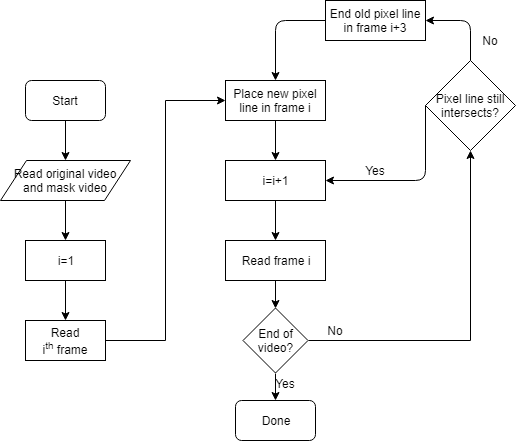
\includegraphics[width=0.9\linewidth]{lineflow.PNG}}
\caption{Pixel line placement flowchart}
\label{lineflow}
\end{figure}

The foreground detection applied can open new opportunity which is detecting object duplication or copy-move. This can be done by simply comparing two foreground's histograms. This again can be done by modifying flood-fill algorithm as shown in Algorithm~\ref{algfloodfillhist}.

\begin{algorithm}
\caption{Pixel line placement}\label{algfloodfillhist}
\begin{algorithmic}[1]
\Procedure{FloodFill}{$node$, $targetcolor$, $replacementcolor$ }
\If{color($node$)$\neq targetcolor$}
  \Return
\EndIf
\State addToHistogram(colorOf($node$))
\State FloodFill(southOf(node), targetcolor, replacementcolor)
\State FloodFill(northOf(node), targetcolor, replacementcolor)
\State FloodFill(westOf(node), targetcolor, replacementcolor)
\State FloodFill(eastOf(node), targetcolor, replacementcolor)
\EndProcedure
\end{algorithmic}
\end{algorithm}

\subsection{Histogram Correlation Calculation}
Calculating correlation between pixel belt will be mostly the same as \cite{b2}. The calculation for spatial tampering detection however need to be redefined. Unlike frames that have linkages between them, foregrounds does not have and thus a full comparison between foregrounds must be performed.

\subsection{Analyzing Correlation}
Inter-quartile range that used in \cite{b2} can be used to analyze the outlier in correlation values. However, to detect spatial tampering, the lower limit $Q1-1.5(Q3-Q1)$ can't be used as a foreground's histogram can be very different from another foreground's histogram and does not imply any tampering done.

\section{Experimental Result}
The proposed method is tested with 18 videos consisting of 4 untampered videos, 8 temporally forged videos, 6 spatially forged videos that downloaded from SULFA dataset \cite{sulfa}. Each video is tested twice in the same environment.

Without foreground detection, the result shows 16 correctly detected and 8 wrongly detected as classified in Table~\ref{tabtdwo}. Meanwhile with foreground detection, the result shows 21 correctly detected and 3 wrongly detected as classified in Table~\ref{tabtdw}. These results show that there is significant improvement from 66.67\% to 87.5\% using foreground detection.

\begin{table}[htbp]
\centering
\caption{Temporal Detection Result Without Foreground Detection}
\begin{tabular}{|c|c|c|}
\hline
& Positive & Negative \\
\hline
True & 13& 3\\
\hline
False & 3& 5\\
\hline
\end{tabular}
\label{tabtdwo}
\end{table}

\begin{table}[htbp]
\centering
\caption{Temporal Detection Result with Foreground Detection}
\begin{tabular}{|c|c|c|}
\hline
& Positive & Negative \\
\hline
True & 16& 5\\
\hline
False & 0& 3\\
\hline
\end{tabular}
\label{tabtdw}
\end{table}

The same experiments were also carried in tampering localization. Without foreground detection, the result shows 10 frames correctly detected and 29 frames wrongly detected as classified in Table~\ref{tabtlwo}. Meanwhile with foreground detection, the result shows 17 correctly detected and 10 wrongly detected as classified in Table~\ref{tabtlw}. These results show that there is significant improvement both from recall that increases from 55.56\% to 94.73\% and from precision from 32.25\% to 66.67\% using foreground detection.

\begin{table}[htbp]
\centering
\caption{Temporal Localization Result Without Foreground Detection}
\begin{tabular}{|c|c|c|}
\hline
& Positive & Negative \\
\hline
True & 10& -\\
\hline
False & 21& 8\\
\hline
\end{tabular}
\label{tabtlwo}
\end{table}

\begin{table}[htbp]
\centering
\caption{Temporal Detection Result with Foreground Detection}
\begin{tabular}{|c|c|c|}
\hline
& Positive & Negative \\
\hline
True & 18& -\\
\hline
False & 9& 1\\
\hline
\end{tabular}
\label{tabtlw}
\end{table}

The significant improvement is obtained from extra process required in the proposed method. This extra process, however, makes significant changes in the time needed to do detection. Without the foreground detection, the average time needed to do detection is 14845.06 ms. Meanwhile, with foreground detection, the average time needed is 20541.94 ms. These results show that there is 38.37\% increased time needed. However, compared to the improvements made, this can be tolerated.

Another experiments using spatially tampered video were also carried and yield 77.78\% accuracy. This result worse than some other method in spatial tampering detection such as cross-correlation method that published in \cite{crosscorrelation} which yield 85\% accuracy. However, the proposed method has 90\% recall that is higher than 82\% recall in \cite{crosscorrelation}.

\begin{table}[htbp]
\centering
\caption{Temporal Detection Result with Foreground Detection}
\begin{tabular}{|c|c|c|}
\hline
& Positive & Negative \\
\hline
True & 9& 5\\
\hline
False & 3& 1\\
\hline
\end{tabular}
\label{tabsd}
\end{table}

\section{Conclusion}
The proposed method improved the method proposed by Jie Xu both in detecting temporally and spatially forged video. The proposed method offers 20.83\% increased accuracy on detecting temporally forged video and 34.42\% increased precision and 39.17\% increased recall on localizing temporally forged video.

The proposed method also makes detecting spatially forged video possible. This method is worse than the other spatial forgery detection method in term of accuracy. However, this method's recall is can be considered better than the others that means the proposed method can identify forgery better.

\begin{thebibliography}{00}
\bibitem{b1} Sowmya K. N and H.R. Chennamma, “A Survey on Video Forgery Detection,” A survey on video forgery detection, vol. 9, no. 2, pp. 17–27, Mar. 2015.
\bibitem{b2} J. Xu, Y. Liang, X. Tian and A. Xie, "A Novel Video Inter-frame Forgery Detection," 2016. 
\bibitem{b3} Christensson, Per. "DV Definition." TechTerms. (2006). Accessed Jan 20, 2019. https://techterms.com/definition/dv.
\bibitem{gmm} McGonagle, John et al. "Gaussian Mixture Model". Brilliant.org. (2015). Accessed Jan 20, 2019. https://brilliant.org/wiki/gaussian-mixture-model/.
\bibitem{sulfa} G. Qadir, S. Yahaya, and A. T. S. Ho, ``Surrey university library for forensic analysis (SULFA) of video content,'' in IET Conference on Image Processing (IPR 2012), 2012.
\bibitem{crosscorrelation} M. Mathai, D. Rajan, and S. Emmanuel, ``Video forgery detection and localization using normalized cross-correlation of moment features,'' 2016 IEEE Southwest Symposium on Image Analysis and Interpretation (SSIAI), 2016.
\vspace{12pt}
\end{thebibliography}

\end{document}
